\documentclass[12pt, a4paper, oneside]{ctexart}
\usepackage{amsmath, amsthm, amssymb, bm, color, graphicx, geometry, mathrsfs,extarrows, braket, booktabs, array}
\usepackage[colorlinks,linkcolor=red,anchorcolor=blue,citecolor=blue,urlcolor=blue,menucolor=black]{hyperref}
\setmainfont{Times New Roman}  % 设置英文字体
\setsansfont{Calibri}
\setmonofont{Consolas}

\linespread{1.4}
%\geometry{left=2.54cm,right=2.54cm,top=3.18cm,bottom=3.18cm}
\geometry{left=1.84cm,right=1.84cm,top=2.18cm,bottom=2.18cm}
\newenvironment{problem}{\par\noindent\textbf{题目. }}{\bigskip\par}
\newenvironment{solution}{\par\noindent\textbf{解答. }}{\bigskip\par}
\newenvironment{note}{\par\noindent\textbf{注记. }}{\bigskip\par}

%%%% 图片相对路径 %%%%
\graphicspath{{figure/}} % 当前目录下的figure文件夹, {../figure/}则是父目录的figure文件夹

\everymath{\displaystyle} % 默认全部行间公式
\DeclareMathOperator*\uplim{\overline{lim}} % 定义上极限 \uplim_{}
\DeclareMathOperator*\lowlim{\underline{lim}} % 定义下极限 \lowlim_{}
\let\leq=\leqslant % 将全部leq变为leqslant
\let\geq=\geqslant % geq同理

% 一些宏定义
\def\bd{\boldsymbol}        % 加粗(向量) boldsymbol
\def\disp{\displaystyle}    % 使用行间公式 displaystyle(默认)
\def\tsty{\textstyle}       % 使用行内公式 textstyle
\def\sign{\text{sign}}      % sign function
\def\wtd{\widetilde}        % 宽波浪线 widetilde
\def\R{\mathbb{R}}          % Real number
\def\N{\mathbb{N}}          % Natural number
\def\Z{\mathbb{Z}}          % Integer number
\def\C{\mathbb{C}}          % Complex number
\def\d{\mathrm{d}}          % differential operator
\def\e{\mathrm{e}}          % Euler's number
\def\i{\mathrm{i}}          % imaginary number
\def\re{\mathrm{Re}}        % Real part
\def\im{\mathrm{Im}}        % Imaginary part
\def\res{\mathrm{Res}}      % Residue
\def\L{\mathcal{L}}         % Loss function
\def\wdh{\widehat}          % 宽帽子 widehat
\def\ol{\overline}          % 上横线 overline
\def\ul{\underline}         % 下横线 underline
\def\bf{\textbf}            % 粗体 textbf
\def\add{\vspace{1ex}}      % 增加行间距
\def\del{\vspace{-3.5ex}}   % 减少行间距

% 基本信息
\newcommand{\RQ}{\today} % 日期
\newcommand{\km}{实变函数} % 科目
\newcommand{\bj}{强基数学002} % 班级
\newcommand{\xm}{吴天阳} % 姓名
\newcommand{\xh}{2204210460} % 学号

\begin{document}

% 正文部分
\section{概述}
\textbf{计算机图形学(Computer Graphics)}: 计算机图形学是研究用计算机表示、生成、处理和显示图形的原理、算法、方法和技术的一门学科.

\textbf{IEEE(电气和电子工程师协会)}: Computer graphics is the art or science of producing graphical images with the aid of computer.

\textbf{ISO(国际标准化组织)}: 计算机图形学是一门通过研究通过计算机将数据转换为图形, 并在专门显示设备显示的原理方法和技术的学科. 它是建立在传统图学理论、应用数学及计算机科学基础上的一门边缘学科.

\section{三维物体的形体几何模型与表示}
\textbf{三维物体几何建模与表示的内涵}: 三维物体\ul{计算机表示的数据结构与存储结构}; 三维物体\\\ul{几何形状数据的存储}.

\subsection{多边形网络模型与表示}
\bf{多边形网络表示的基本单元}: \ul{多边形平面}.

\bf{多边形平面的定义}: 由\ul{空间点集(顶点)}和\ul{点之间的拓扑关系(边)}定义.

足够多的多边形平面可以无限逼近三维物体表面几何形体. 

\bf{物体表面特征}: \ul{透明度、表面反射系数、纹理坐标等}, 可用多边形网络的\ul{顶点属性、}\\\ul{边属性和多边形属性}所定义.

多边形网格表示要求满足\bf{一致性约束}.

\bf{多边形网格表示的概念}: \ul{层次分解}与\ul{存储结构设计}.

\bf{多边形网格表示的基本特点}: \ul{构造简单}, 可表示任意三维物体表面几何形体; 已形成完善有效的\ul{明暗处理方法、硬件可实现}; 表面几何形体\ul{表示精度与多边形网格数量成正比}; \\\ul{表示精度可伸缩}是多边形网络模型的\bf{追求}; \ul{可编辑}是多边形网格表示的\bf{挑战}.

\subsection{曲面片模型与表示}
曲面片\bf{由精确参数表示}, 其面上的每个点都有定义; 具有\bf{三维形状编辑能力}, 是\ul{CAD交互式}\\\ul{设计基础}; \bf{可能是一种更经济}的物体几何形状表示法.

\subsection{构造实体几何模型(CSG: Constructive Solid Geometry)}
CSG使用\bf{三维基本构造块}组合构建的一种\bf{三维物体形体层次表示}. CSG是一种分解表示的\bf{有序二叉树}, \ul{叶子节点}是\bf{体素}或\bf{形体变换参数}, \ul{分支节点}是\bf{正则集合运算}或\bf{几何变换操作}. \ul{构造实体几何表示}流行于\ul{交互式CAD领域}.

\bf{CSG模型表示的主要特点}: \ul{正则集合运算(正则并、正则交、正则差)和集合变换}描述三维物体组成过程; \ul{隐含表示形体几何边界元素}; 需\ul{特殊绘制或多边形网络转换}; 支持实现\ul{交互式}\\\ul{实体建模}.

\subsection{空间细分表示}
把三维物体所在的整个\ul{世界空间细分为更小的立方体基元}, 按\ul{是否在物体中标记}每一个\bf{体素(Voxel)}. 体素的数据组织存储是\bf{八叉树}, 八叉树编码可用于\ul{表示三维实体内部的分层树形结构}. 八叉树保持\ul{体素空间信息以及稀疏性}, 可以转换为\ul{二叉空间分区树(BSP)}.

虽然三维物体表示的选择和使用受多种因素影响, 但考虑技术成熟度和计算资源, \bf{多边形网络}是交互图形引擎\bf{最普及}支持的三维物体表面几何形体表示模型.

\section{三角网格的几何计算}
\subsection{三角网格及其存储表示}
三角网络模型用三角形组成的\bf{面片列表}近似三维物体表面几何形体.

三角网络模型的两种典型存储: 三角形网络模型的\bf{线性表结构}--obj文件格式; 三角网格模型的\bf{双向链表边表结构}(half-edge半边结构).

\subsection{三角网格的生成}

现有\bf{传感器获取}物体表面离散点的\ul{空间坐标}, 对区域内的一组给定点, \bf{Voronoi(沃若诺依)图}是对区域内给定一组基点的\ul{单元分区}; \bf{Delaunay(德洛内)三角剖分}完成区域内对给定基点的拓扑连接, \ul{形成三角形闭合平面}.


\bf{三角网格生成的本质}: 将\ul{三维物体表面划分为一组三角形面片}.

(1) Voronoi图生成的\bf{泰森法}: 1. 构建Delaunay三角形; 2. 选择一个点的所有相关三角形; 3. 计算每个三角形的外接圆心; 4. 连接圆心.

(2) 二维平面Delaunay三角剖分的\bf{空圆特性}: 两个共边三角形, 任意一个三角形的外接圆中都不能包含另一个三角形的顶点.

(3) 二维平面Delaunay三角剖分的增量构造算法, \bf{Lawson算法}: 先构造一个超级三角形, 然后每次插入一个点, 找到外接圆包含它的三角形, 删除公共边, 在全部连起来, 过程如下图.
\begin{figure}[htbp]
    \centering
    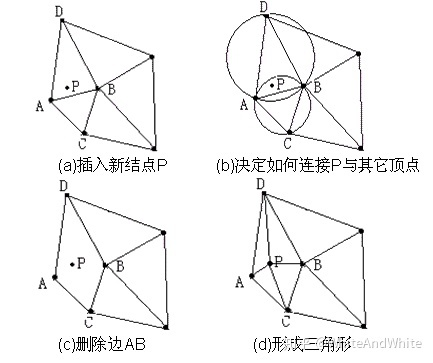
\includegraphics[scale=0.6]{lawson.jpg}
\end{figure}

\subsection{网格简化}
在\bf{保持}三角形网格对三角形物体表面形体几何\bf{逼近条件}下, \ul{减少网络的顶点、边和多边形}\\\ul{面片数量}.

网络简化的三种技术: \bf{顶点删除法、边折叠法和面片收缩法}.

\subsection{网络细分}
用更多的\bf{较小网格面}代替原有曲面, 更加逼近物体表面几何形状. 需要确定\bf{几何规则}和\bf{拓扑规则}:

\bf{几何规则}: 用于计算新顶点\bf{位置}.

\bf{拓扑规则}: 用于确定新顶点的\bf{连接关系}.

\bf{Loop细分(一种细分算法)}: 1-4三角形分裂法, 即将一个三角形面片分为四个新三角形面片. 思想: 将三角形的每个边上新增一个顶点, 把同一三角形内的新增顶点连接组成四个三角形(如下图所示).

\begin{figure}[htbp]
    \centering
    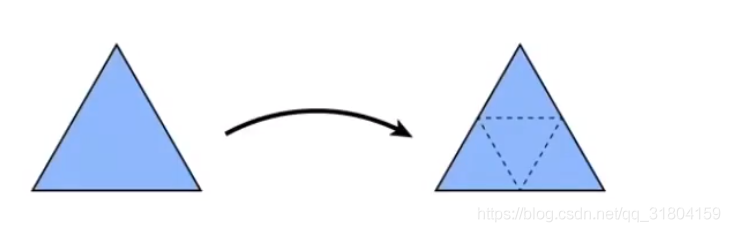
\includegraphics[scale=0.4]{loop.png}
\end{figure}

\section{多边形网格的三维物体绘制}
\subsection{多边形网格渲染流水线}
\bf{渲染流水线}是指\ul{将多边形网格表示的三维物体表面形体}转化为能在\ul{设备上显示的}、经过明暗处理的\ul{像素亮度计算}过程.

涉及模型\ul{坐标空间、世界坐标空间、观察坐标空间、设备坐标空间}.

对应三维物体的\ul{模型变换、观察变换和投影变换}.

\subsection{可见面判定和隐藏面消除}
由于投影变换使得三维物体失去了深度信息, 真实感绘制必须\bf{消除被遮挡的不可见线或面}, 在\ul{二维显示设备}中\bf{将三维物体的可见面表示出来}.

Z缓存算法(Z-buffer): \bf{最简单的可见面判定算法};

光线投影算法: \bf{最自然的消隐算法};

深度排序算法(画家算法): \bf{最偷懒的消隐算法}.

\subsection{多边形网格裁剪}

\bf{网格裁剪的理由}: 显示设备的视窗大小固定, \bf{显示实体范围有限}, \bf{避免无效计算}, 节省计算资源.

(1) \bf{二维直线段裁剪}: Cohen-Sutherland; 梁友栋-Barsky; Nicholl-Lee-Nicholl.

(2) \bf{二维多边形裁剪}: Sutherland-Hodgeman, 问题: 对凹多边形裁剪可能会产生多余的边.

(3) \bf{三维视见体与三维线段裁剪}: 定义端点6位区域编码的三维线段裁剪方法.

\section{图元的光栅化计算}
\subsection{数学图元的像素扫描转换}

讨论将\bf{无限点构成的数学图元}转化到\bf{有限像素图形逼近}的扫描变换方法.

(1) \ul{直线扫描转换}的\bf{基本增量算法}. (数值微分DDA法)

(2) \ul{直线扫描转换}的\bf{中点线算法}.

(3) \bf{Bresenham(布雷森汉姆)}\ul{直线扫描转换}算法.

(4) \bf{中点画圆法}.

\subsection{多边形扫描转换与区域填充}

\bf{多边形扫描转换}对\ul{多边形形状无限制}, 但多边形边界必须是\bf{封闭的}, 且\bf{不自交的}.

典型的三种多边形: \bf{凸多边形、凹多边形、内含环多边形}.

\bf{多边形扫描线填充算法}: 按照扫描线顺序计算\ul{计算相交区间}, 设置区间像素的\ul{亮度值}. 过程如下:

(1) \bf{求交}: 计算扫描线与多边形各边的交点;

(2) \bf{排序}: 把所有交点按x值递增排序;

(3) \bf{配对}: 确定交点对, 区分扫描线与多边形的一个相交区间;

(4) \bf{着色}: 把相交区间内像素设置为指定颜色.

\begin{figure}[htbp]
    \centering
    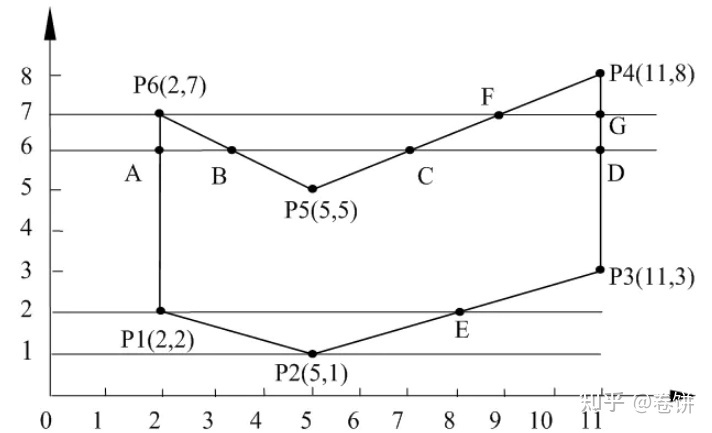
\includegraphics[scale=0.4]{多边形扫描线填充.jpg}
\end{figure}

\subsection{走样与反走样}

\bf{走样}: 在光栅显示中, 用\ul{离散量表示连续量}引起的\bf{失真现象}.

\bf{反走样}: 减轻或除去走样的技术.

\bf{反走样基本策略}: \bf{提高分辨率}(\ul{子像素}是方法之一), \bf{像素采用不同的灰度值}(\ul{加权区域采样}是确定像素灰度值的方法之一).

\section{局部光照模型与明暗处理}

讨论绘制图像的\bf{像素亮度计算原理与方法}. \bf{局部光照模型}是计算三维物体表面光强度的物理依据.

\subsection{局部光照模型: 像素级光强计算}

\bf{局部光照模型}是建立在\ul{物体不透明}, 仅考虑\ul{光源直接照射物体表面}时的\ul{光传播过程}.

模拟物体表面光的传播包括: \bf{入射光, 环境光, 理想漫反射光, 非理想镜面反射光}.

影响物体光强表面光强的因素包括: \bf{物体表面几何形状, 光源, 环境(遮挡, 反射与折射), 视点位置, 物体表面属性(材料, 光洁度等)}.

(1) 简单光照模型 - 环境光.

(2) 理想漫反射模型.

(3) 非理想镜面反射模型.

(4) Phong(裴祥风)光照明模型.

\subsection{插值明暗处理: 多边形表面光强计算}

\bf{插值明暗处理}是在对象空间以\bf{多边形为基本单元}计算\ul{物体表面的光强度}.

仅仅按像素亮度计算会产生\bf{马赫带效应}, 插值明暗处理方法可以避免邻接多边形间的\\\ul{光强不连续性(发生走样)}.

(1) Gouraud(高洛德)明暗处理方法.

(2) Phong明暗处理方法.

\section{表面纹理映射技术}

\bf{表面纹理映射技术}能够丰富物体表面细节的真实感.

\bf{颜色纹理}: 各种\bf{花纹、图案和文字}, 如大理石墙面、字画、器皿图案等图像数据.

\bf{几何纹理}: 基于景物表面\bf{微观几何形状的表面纹理}, 如桔子、树干、岩石等表面呈凸凹不平的纹理细节.

\bf{过程纹理}: 表现\bf{各种规则或不规则动态变化自然景象}, 如水波、云、火、烟雾.

\subsection{二维纹理映射过程}

\bf{二维纹理映射过程}: 将\ul{二维纹理图像}映射到\ul{三维物体空间}, 再将\ul{物体投影到屏幕空间}的变化过程.

\bf{本质}: 建立\ul{纹理空间与物体空间}的映射关系.

\bf{反向映射}: 借助物体空间与纹理空间的映射关系, 实现观察平面空间的像素求值.

纹理空间坐标计算方法: (1) 双线性插值法; (2) 中间表面法.

\bf{S映射}: 完成\ul{纹理空间与三维中间表面空间}的映射.

\bf{0映射}: 进行\ul{中间表面与物体空间}的关联映射.

\subsection{凹凸映射技术}

问题: 对物体表面采取微小扰动, 从而引起物体表面法向变化, 导致表面光亮度计算值突变.

解决: 利用人类视觉的\bf{马赫带效应}从而产生表面凸凹不平的真实感绘制渲染效果.

(1) 几何扰动法. (2) 法向扰动法.

实例: 特定人脸网络模型重建与纹理映射算法应用.

\section{几何阴影生成}

几何阴影强化物体间空间关系, 增加绘制图像的立体感和场景真实感.

(1) 投影多边形/扫描线方法.

(2) 阴影体算法.

(3) 从光源变换导出阴影多边形方法.

(4) 阴影Z缓冲器算法.

\section{全局光照模型}

考虑环境\bf{漫反射、镜面反射和规则投射}对景物表面产生的\bf{整体照明效果}.

物体表面入射光的构成: \bf{光源直接照、其他物体的反射光、透射光}.

模拟光照全局交互方法:

1. \bf{光线追踪法}, 关注\ul{物体表面的完全镜面交互}, 从光源开始, \ul{跟踪每一条光的路径穿过环境}, \\\ul{直到光线击中视点为止};

2. \bf{辐射度方法}, 关注\ul{物体表面的完全漫反射交互}, 假设\ul{光能在所有方向上进行等量反射},\\\ul{形成一个以反射点为中心的半球}.

\subsection{Whitted光线追踪方法}

模拟物体表面的\bf{镜面反射、规则透视和光源直射的全局光照效果}. 适用于光滑表面, 非光滑表面不理想.

\subsection{光能辐射度方法}

基本原理: 1. \bf{能量守恒}; 2. 整个封闭空间的\bf{光能分布达到平衡状态}; 3. 场景的\bf{明暗变化}反映了场景各面片\bf{辐射度的大小的变化}.

局限性: 1. 场景中的镜面物体不能用辐射度绘制处理; 2. 使用辐射度方法前, 场景必须被离散化.

\section{三维曲线与曲面表示}

\subsection{曲线与曲面的参数表示}

\bf{样条(spline)}: 由多个曲线段连接而成的复合曲线;

\bf{插值样条曲线}: 给定\ul{一组有序控制点}构造的一条\ul{顺序通过这些控制点的曲线}.

\bf{逼近样条曲线}: 给定\ul{一组有序控制点}构造的一条\ul{在某种意义下最接近控制点的曲线}(不一定通过控制点).

\bf{样条曲线段的连续性条件}: \ul{参数连续性、几何连续性};

\bf{参数曲线曲面的三种等价数学描述}: \ul{边界条件、特征矩阵和基函数}表示.

\subsection{典型三次插值样条曲线}

\subsubsection{自然三次样条曲线}

给定$n+1$个控制点, 通过$n$个三次多项式曲线通过控制点, 相邻曲线段在连接点处有相同的一阶和二阶导数.

\subsubsection{Hermite样条曲线}

由给定控制点和每个控制点\bf{切向量约束}, 确定的通过每个控制点的分段三次多项式曲线, 构成一条Hermite样条曲线.

\subsubsection{Cardinal样条曲线}

不同余Hermite样条曲线, Cardinal样条控制点的\bf{切向量正比于两个相邻控制点形成的弦}, 引入一个\bf{张量参数}控制\ul{样条与输入控制点间的松弛度}.

三次Bezier(贝塞尔)曲线和B样条曲线是两种典型的三次逼近样条曲线.

\subsection{Bezier曲线}
Bezier曲线将\bf{函数逼近论和集合表示结合}, 使用一定数目控制点构造参数曲线.

三次Bezier曲线的基函数表示和基本特性;

三次Bezier曲线段拼接的复杂样条曲线构造;

抛物线三切线定理;

三次Bezier曲线的集合作图法涵义和曲线上点的递推计算方法.

\subsection{B样条曲线}

B样条的曲线\ul{多项式次数独立于控制点数目}, \ul{多项式系数由少数几个控制点决定}, 具有\bf{局部控制性}.

三次B样条曲线的基函数表示、B样条曲线的基本特性;

三次B样条曲线段拼接的复杂样条曲线构造;

B样条曲线类型: \bf{均匀B样条曲线、准均匀B样条曲线、非均匀B样条曲线}.

\subsection{Bezier曲面}

三维曲面: 两条曲线的笛卡尔积产生.

双三次Bezier曲面片的参数表示, 曲面片的连接.

% 下面给一些功能的写法
\iffalse
% 图片模板
\centerline{
    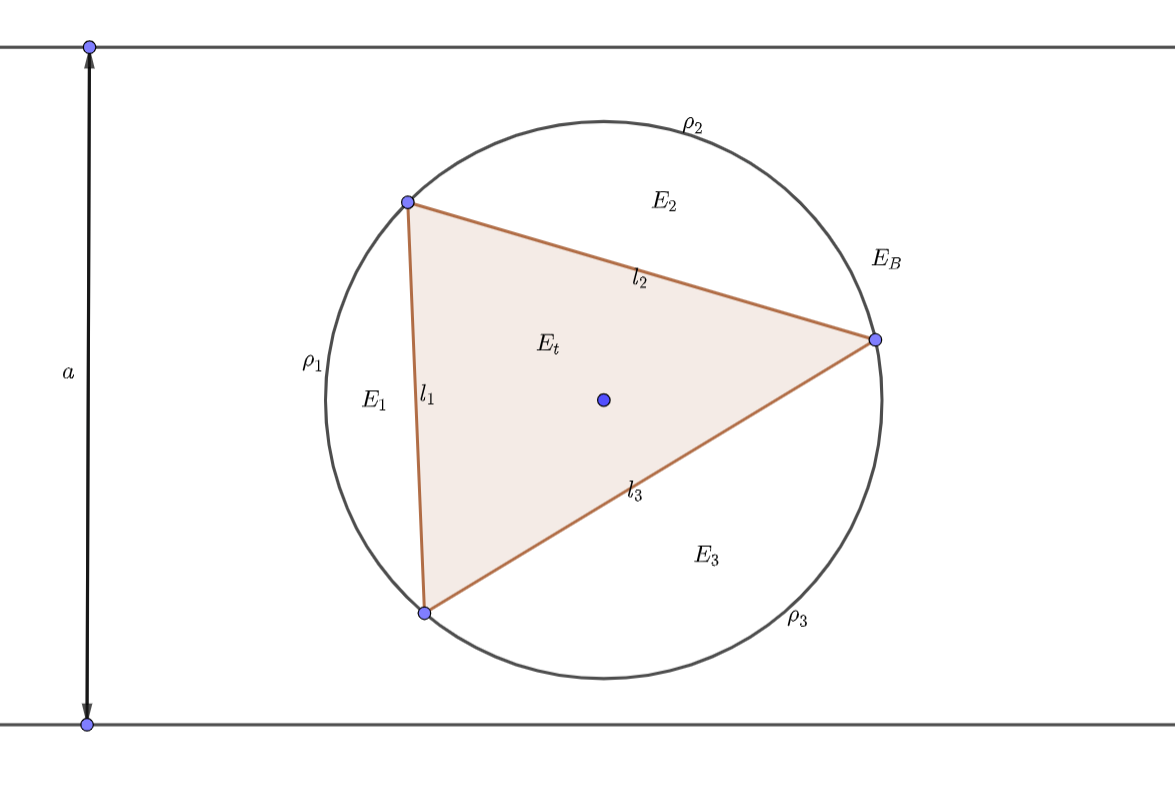
\includegraphics[width=0.8\textwidth]{figure.png}
}
% 表格模板
\renewcommand\arraystretch{0.8} % 设置表格高度为原来的0.8倍
\begin{table}[!htbp] % table标准
    \centering % 表格居中
    \begin{tabular}{p{1cm}<{\centering}p{1cm}<{\centering}p{3cm}<{\centering}p{5cm}<{\centering}} % 设置表格宽度
    %\begin{tabular}{cccc}
        \toprule
        $x_i$ & $f[x_1]$ & $f[x_i,x_{i+1}]$ & $f[x_i,x_{i+1},x_{i+2}]$ \\
        \midrule
        $x_0$ & $f(x_0)$ &                  &                          \\
        $x_0$ & $f(x_0)$ & $f'(x_0)$        &                          \\
        $x_0$ & $f(x_1)$ & $\frac{f(x_1)-f(x_0)}{x_1-x_0}$ & $\frac{f(x_1)-f(x_0)}{(x_1-x_0)^2}-\frac{f'(x_0)}{x_1-x_0}$\\
        \bottomrule
    \end{tabular}
\end{table}

\def\Log{\text{Log}} % 一个简单的宏定义
$\Log$ % 调用方法
\fi

\end{document}